\chapter{Brugermanual}

I dette afsnit vil vi beskrive en simpel brugermanual til spillet. Vi vil fokusere på den primære styringsmetode vha. rattet og gearstangen. Spillet kan dog også spillet vha. computerens keyboard eller knapperne på microcontrolleren.
\\

Det første der møder en når man starter spillet er skærmbilledet der ses på figur \ref{fig:startup}. Den blinkende tekst under logoet angiver at brugeren skal trykke på en valgfri tast for at starte spillet. ASCII arten af rattet skulle gerne give en indikation af hvordan spillet styres. Et billede af rattet til sammenligning kan ses i figur \ref{fig:rat_med_controls}.\\
\newpage

\begin{figure}[h!]
\begin{minipage}[b]{0.49\textwidth}
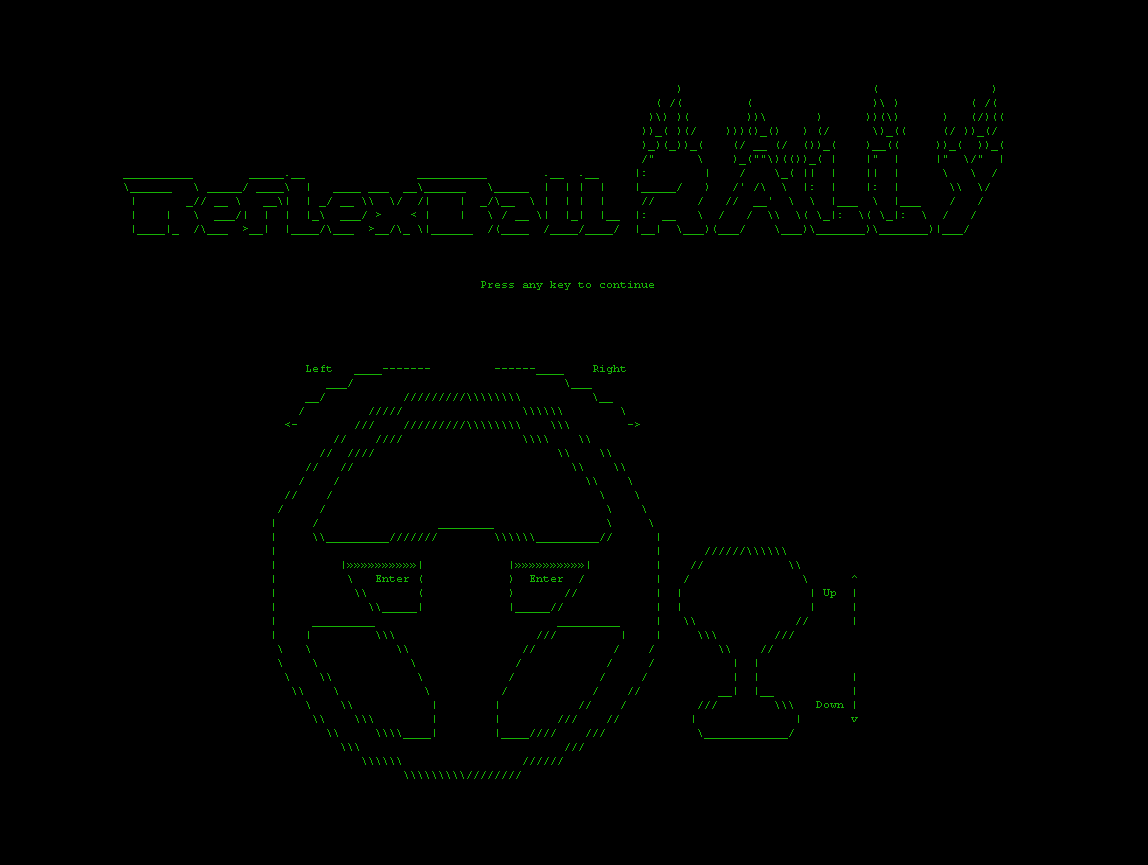
\includegraphics[width=\linewidth]{figs/screenshots/startup_crop_ny.png}
\caption{Screenshot af startup skærmen}
\label{fig:startup}
\end{minipage}\hfill
\begin{minipage}[b]{0.49\textwidth}
\includegraphics[width=\linewidth]{figs/rat_med_controls.png}
\caption{Oversigt over styring af rattet}
\label{fig:rat_med_controls}
\end{minipage}\hfill
\end{figure}

Derefter vises menuen svarende til den i figur \ref{fig:menu_2}. Her kan brugeren vælge sværhedsgraden. Brugeren kan således flytte bolden op og ned vha. gearet. Når den ønskede sværhedsgrad er valgt kan spillet startes ved at trykke på en af de to knapper der sidder på rattet. Den valgte sværhedsgrad bestemmer derefter bredden af strikeren, samt hvor hurtigt bolden skal begynde at forøge sin hastighed jo sværre mode, jo hurtigere forøges boldhastigheden. Ved valg af Chuck Norris mode er boldens hastighed dog den maksimale fra starten. For mere information henvises til funktionen \nameref{asciidisplay} i appendiks \ref{C kode}. \\

\begin{figure}[h!]
\centering
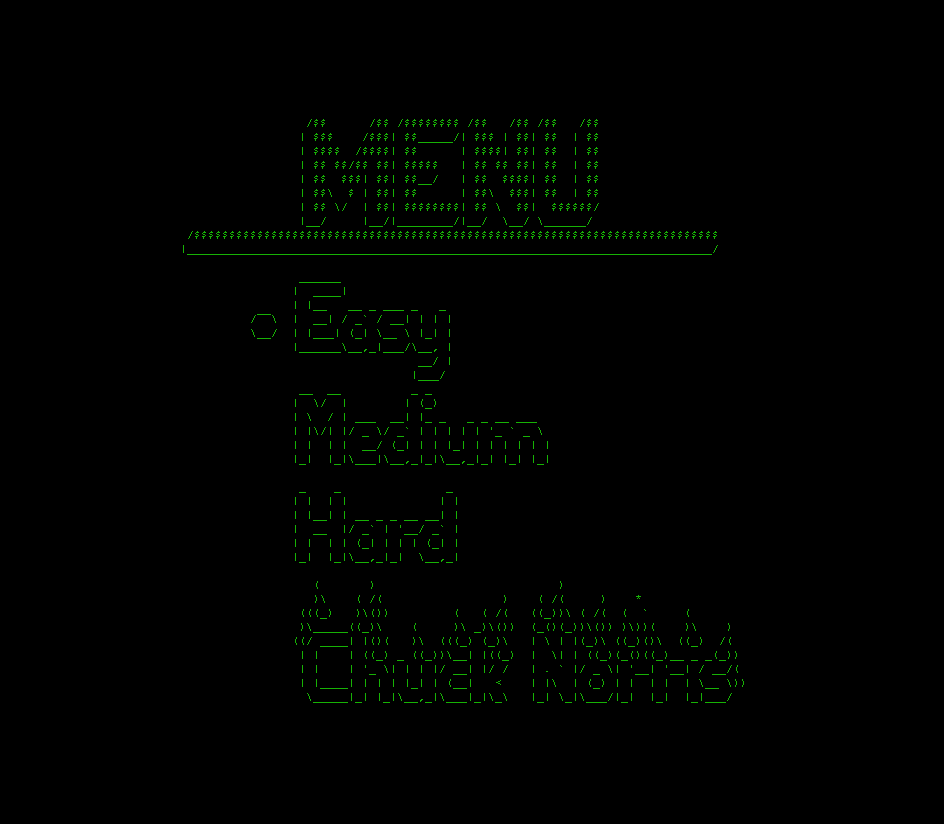
\includegraphics[scale=0.25]{figs/screenshots/menu_crop.png}
\caption{Screenshot af menuen}
\label{fig:menu_2}
\end{figure}

Efter dette begynder selve spillet. Når spillet starter har man 3 liv og for hver gang det ikke lykkes en at fange bolden med strikeren, inden den ryger forbi, mister man et liv. Man skyder bolden afsted ved enten af at hive gearstangen tilbage eller trykke på en af de to knapper på rattet. Bolden vil da skydes afsted med en vilkårlig vinkel på 45-135 grader. Herefter gælder det blot om at skyde alle brikkerne ned ved at bevæge strikeren ved at dreje på rattet. Der er forskellig afbøjningsvinkel afhængigt af hvor bolden rammer strikeren. En god spiller kan bruge dette til at få bolden afbøjet i den retning han/hun gerne vil.\\

Hver gang brugeren rammer en brik fås 1 point. Bemærk at det ikke giver point når strikeren rammer bolden, så det belønner sig ikke at forlænge banen, ved at sørge for ikke at ramme brikker. Scoren bliver løbende vist på LED displayet på microcontrolleren så længe man er i live. Hvis man dør scrolles pointene ud på LED displayet og derefter scrolles antal liv man har tilbage igennem og til sidst scrolles pointene frem igen og stopper når de udfylder hele displayet, se figur \ref{fig:board_overview}. Hvis man er utålmodig og ikke kan vente til der er scrollet færdig kan man sagtens starte spillet imens.\\

Hvis brugeren skyder alle brikkerne i stykker avancerer brugeren til næste level og får som belønning 2 ekstra liv. Her vil LED displayet begynde at scrolle. Først kommer beskeden "Level up!", dernæst scrolles hvilket level man er nået til igennem, så hvor mange liv man nu har og til sidst scrolles pointene tilbage ind igen. Når en ny bane påbegyndes nulstilles boldens hastighed til starthastigheden på den givne sværhedsgrad. Men pas på, banerne bliver sværere og sværere!\\

Et overblik over alle de 6 levels i spillet kan ses på figurerne nedenfor. Bemærk at der i level 6 er en hel udfyldt række af usynlige brikker, der først bliver synlige når man har ramt dem én gang. Disse brikker har 5 liv og er derfor væsentligt sværere at slå i stykker. Se \nameref{levels} i appendiks \ref{C kode}. \\

\begin{figure}[h!]
\begin{minipage}[b]{0.32\textwidth}
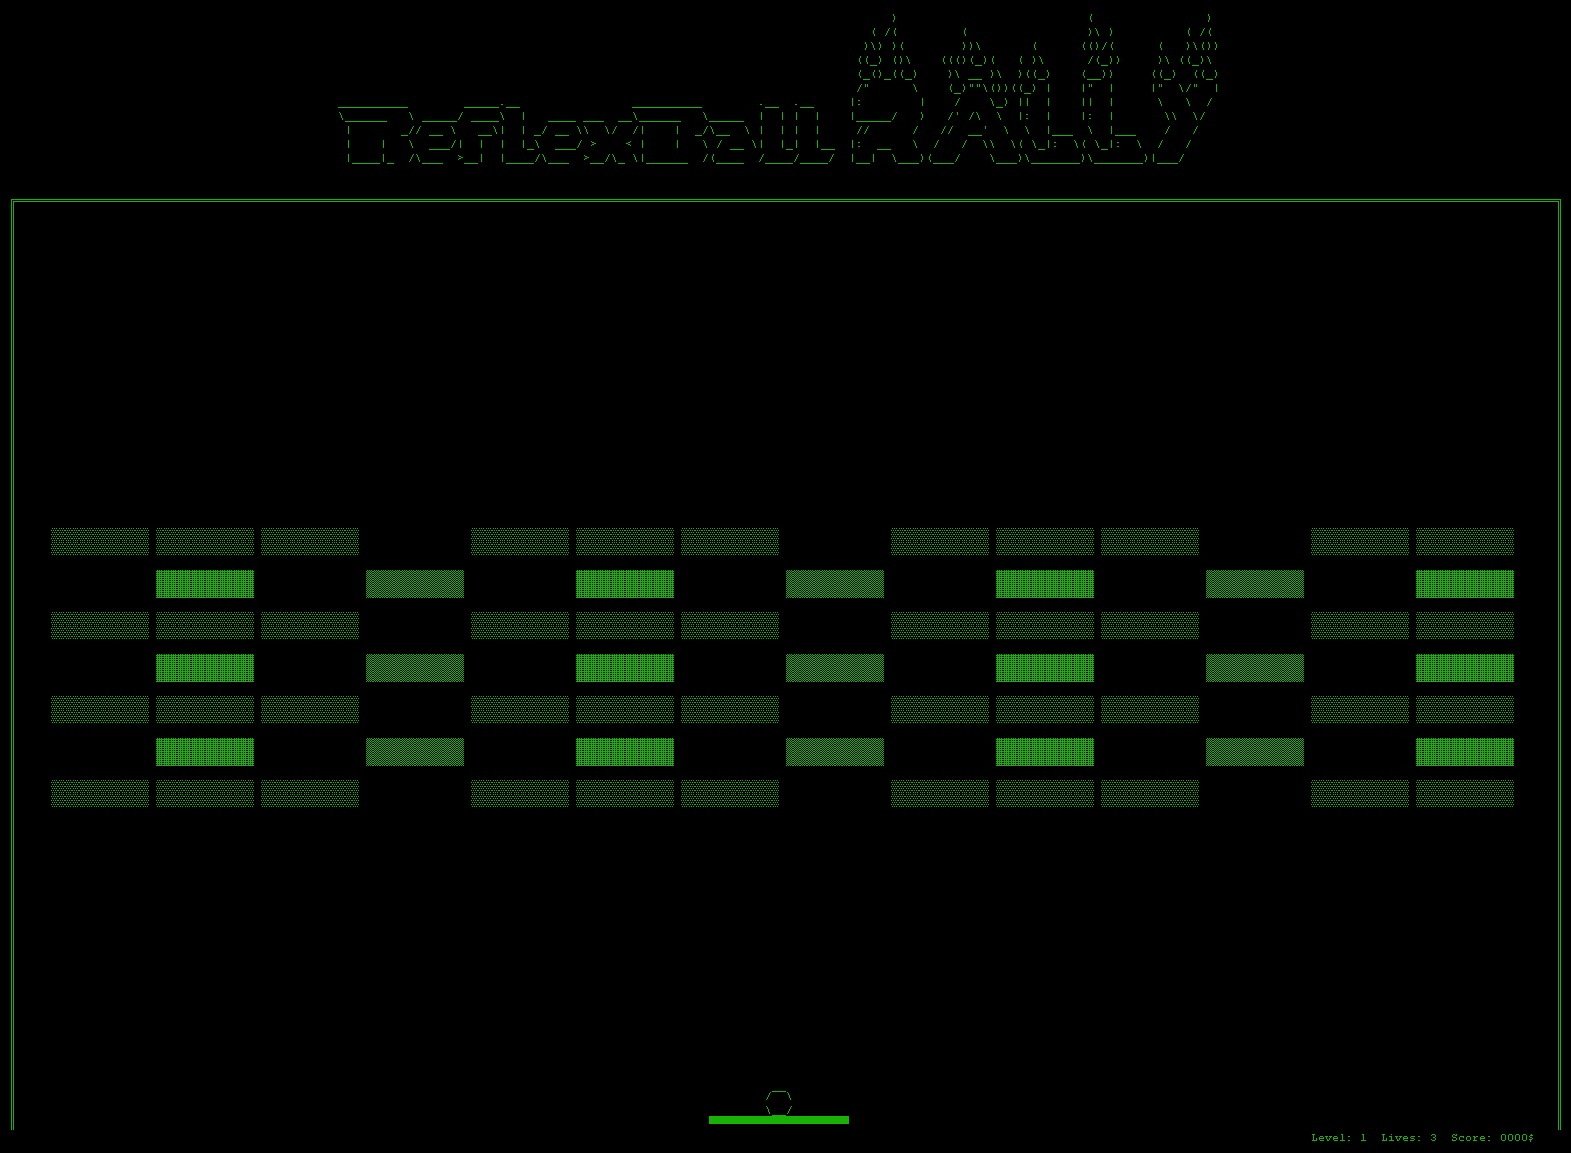
\includegraphics[width=\linewidth]{figs/screenshots/level1.png}
\caption{Level 1}
\label{fig:level1_2}
\end{minipage}\hfill
\begin{minipage}[b]{0.32\textwidth}
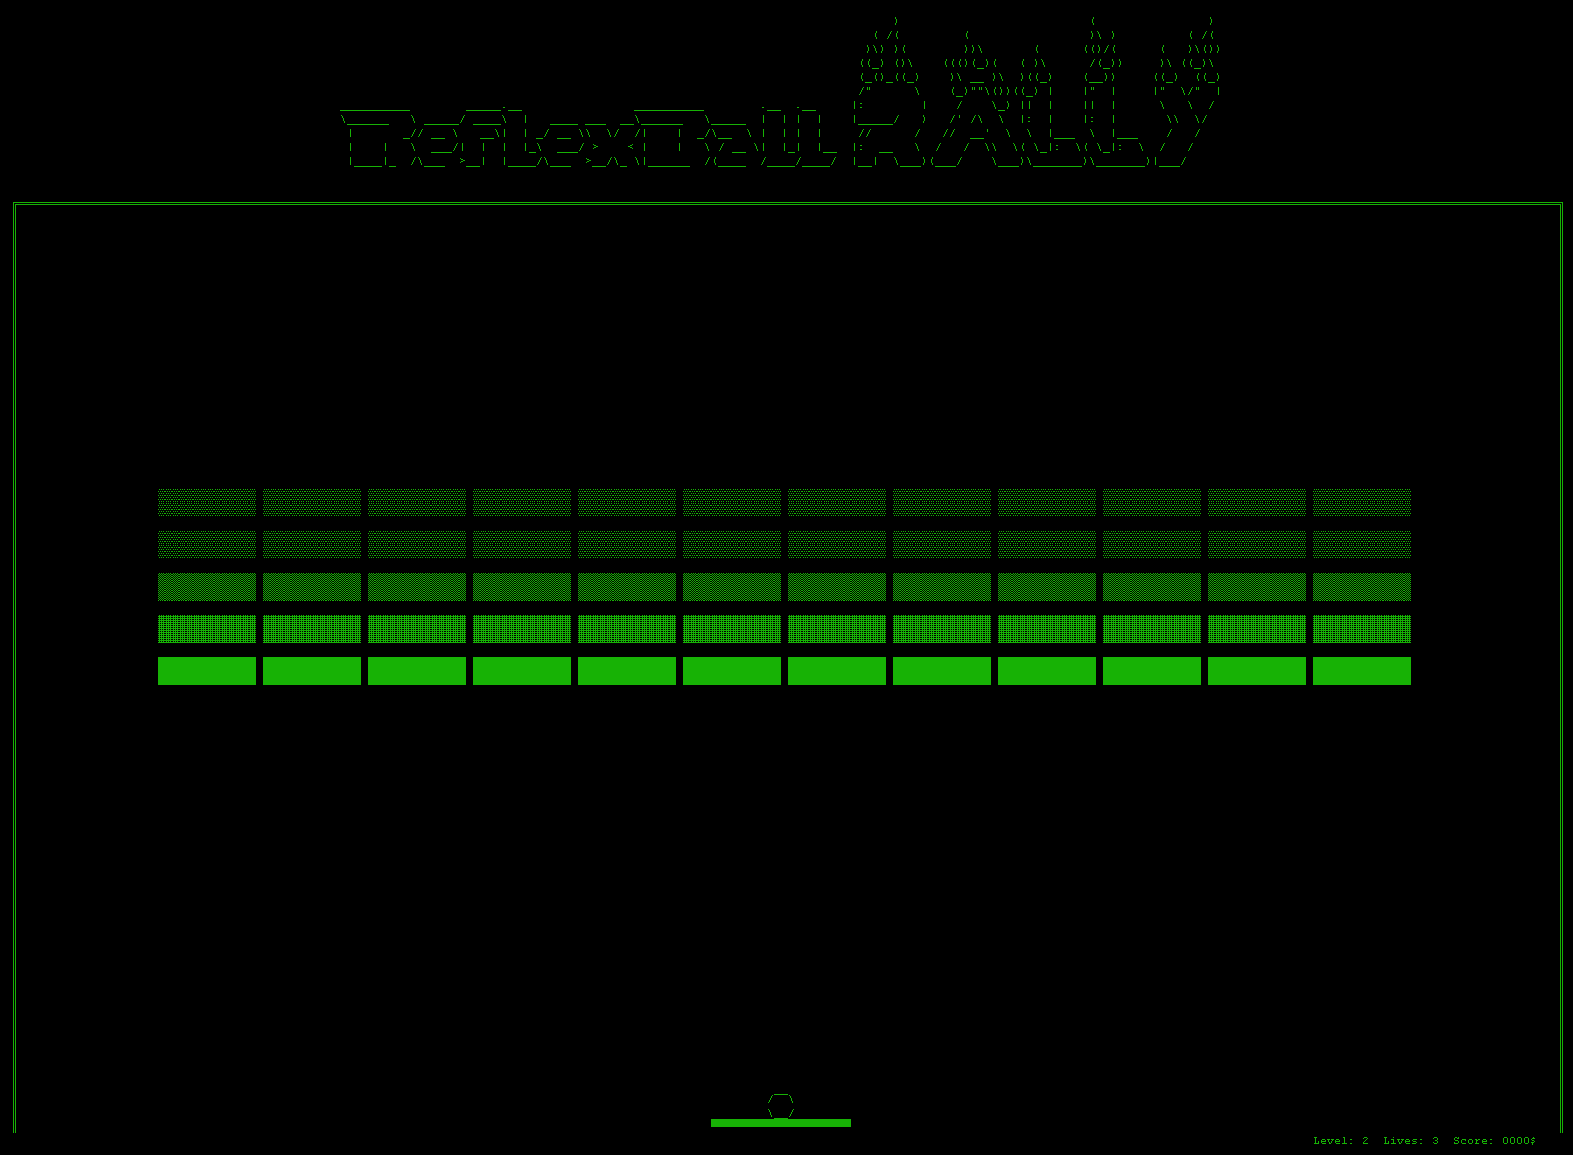
\includegraphics[width=\linewidth]{figs/screenshots/level2.png}
\caption{Level 2}
\label{fig:level2}
\end{minipage}\hfill
\begin{minipage}[b]{0.32\textwidth}
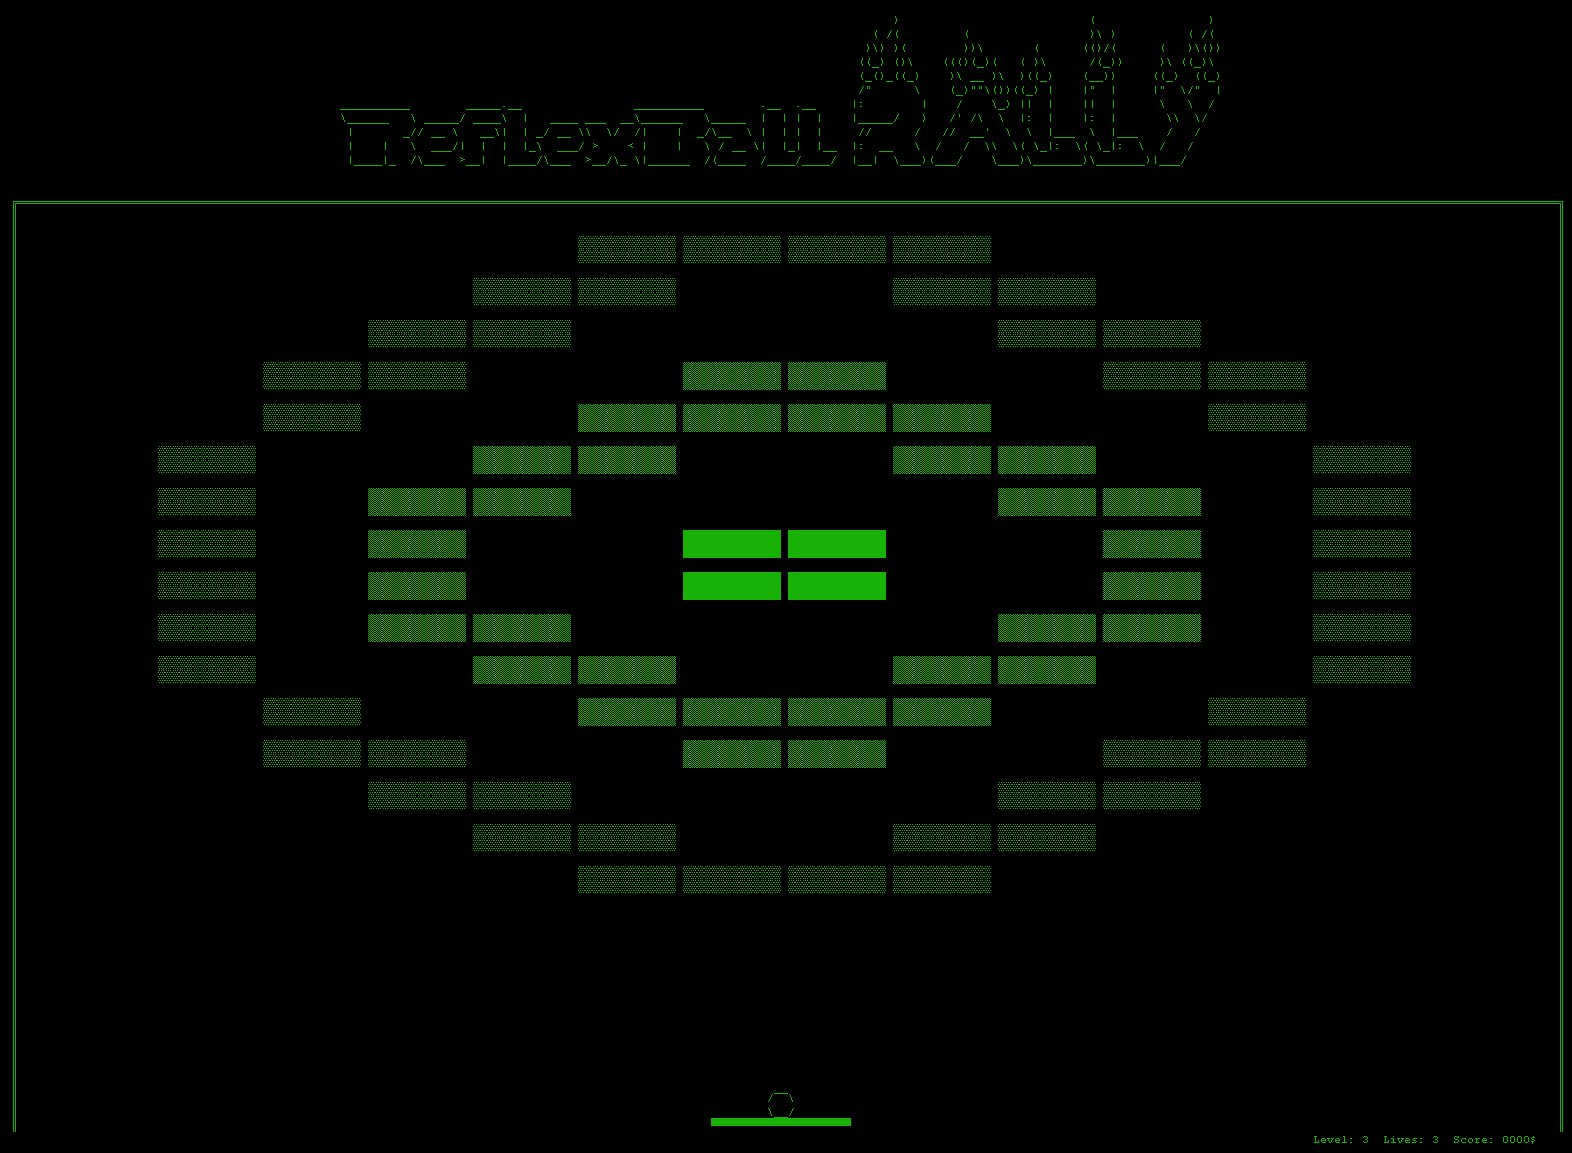
\includegraphics[width=\linewidth]{figs/screenshots/level3.png}
\caption{Level 3}
\label{fig:level3}
\end{minipage}\hfill
\begin{minipage}[b]{0.32\textwidth}
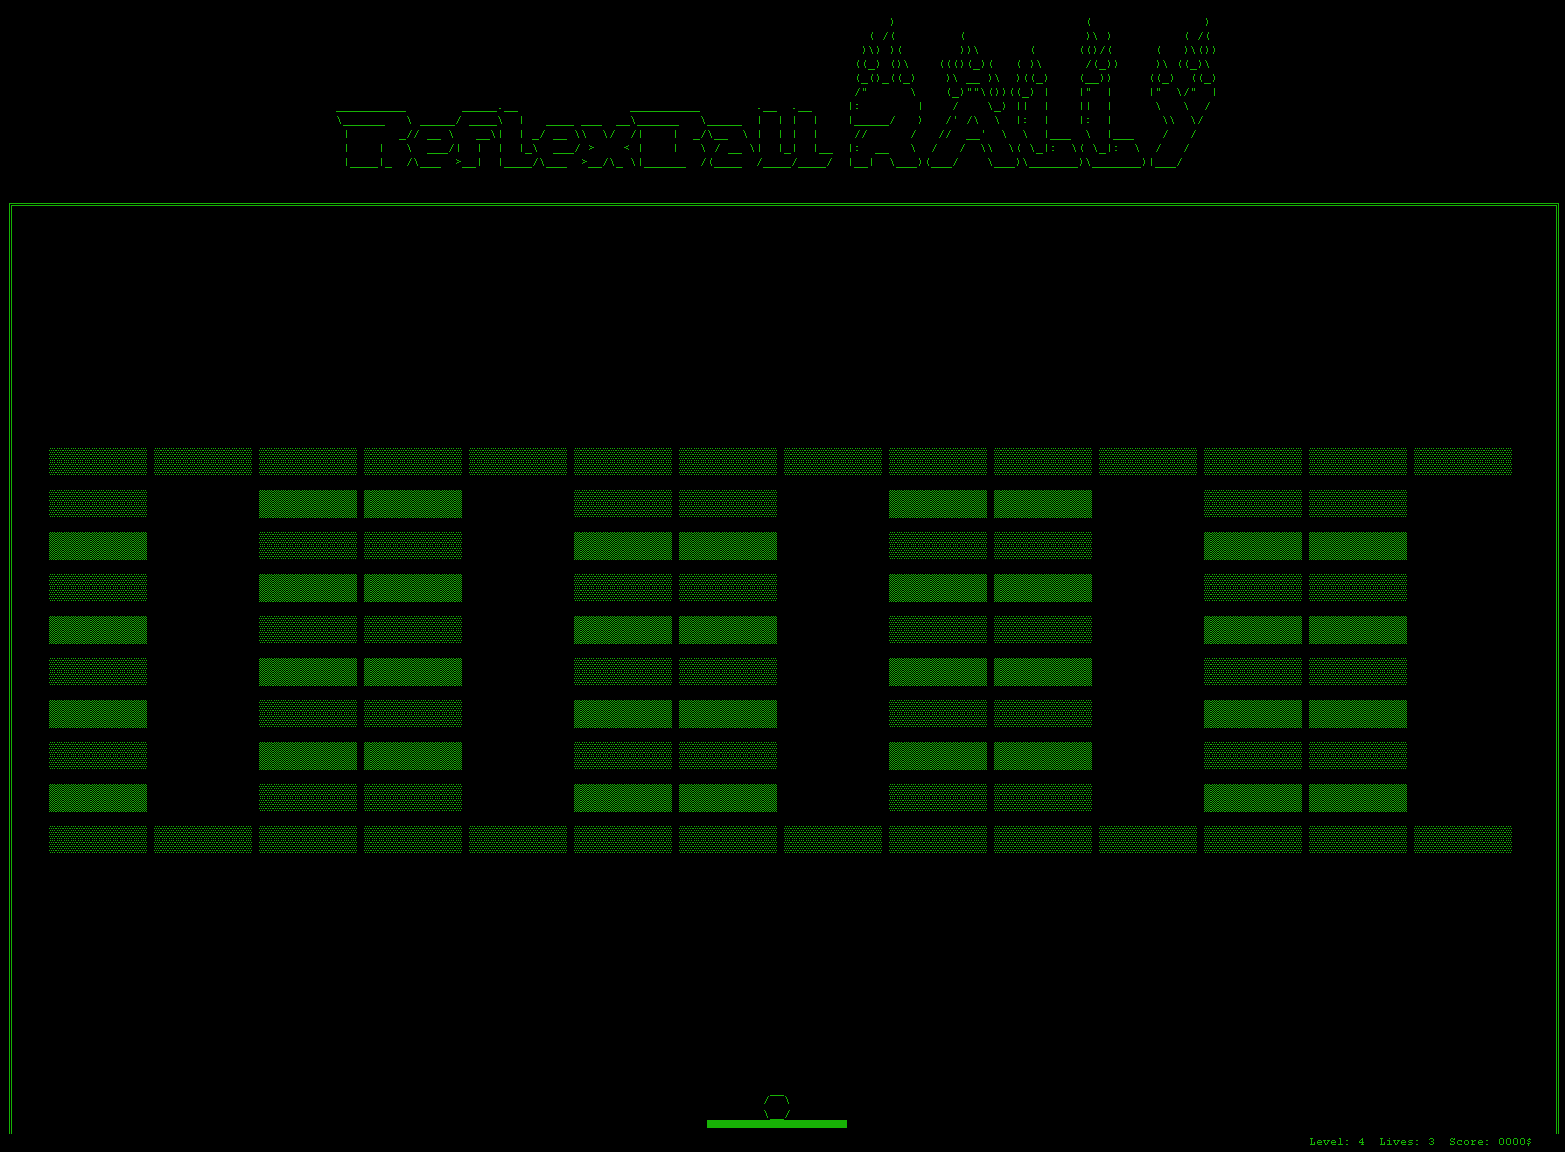
\includegraphics[width=\linewidth]{figs/screenshots/level4.png}
\caption{Level 4}
\label{fig:level4}
\end{minipage}\hfill
\begin{minipage}[b]{0.32\textwidth}
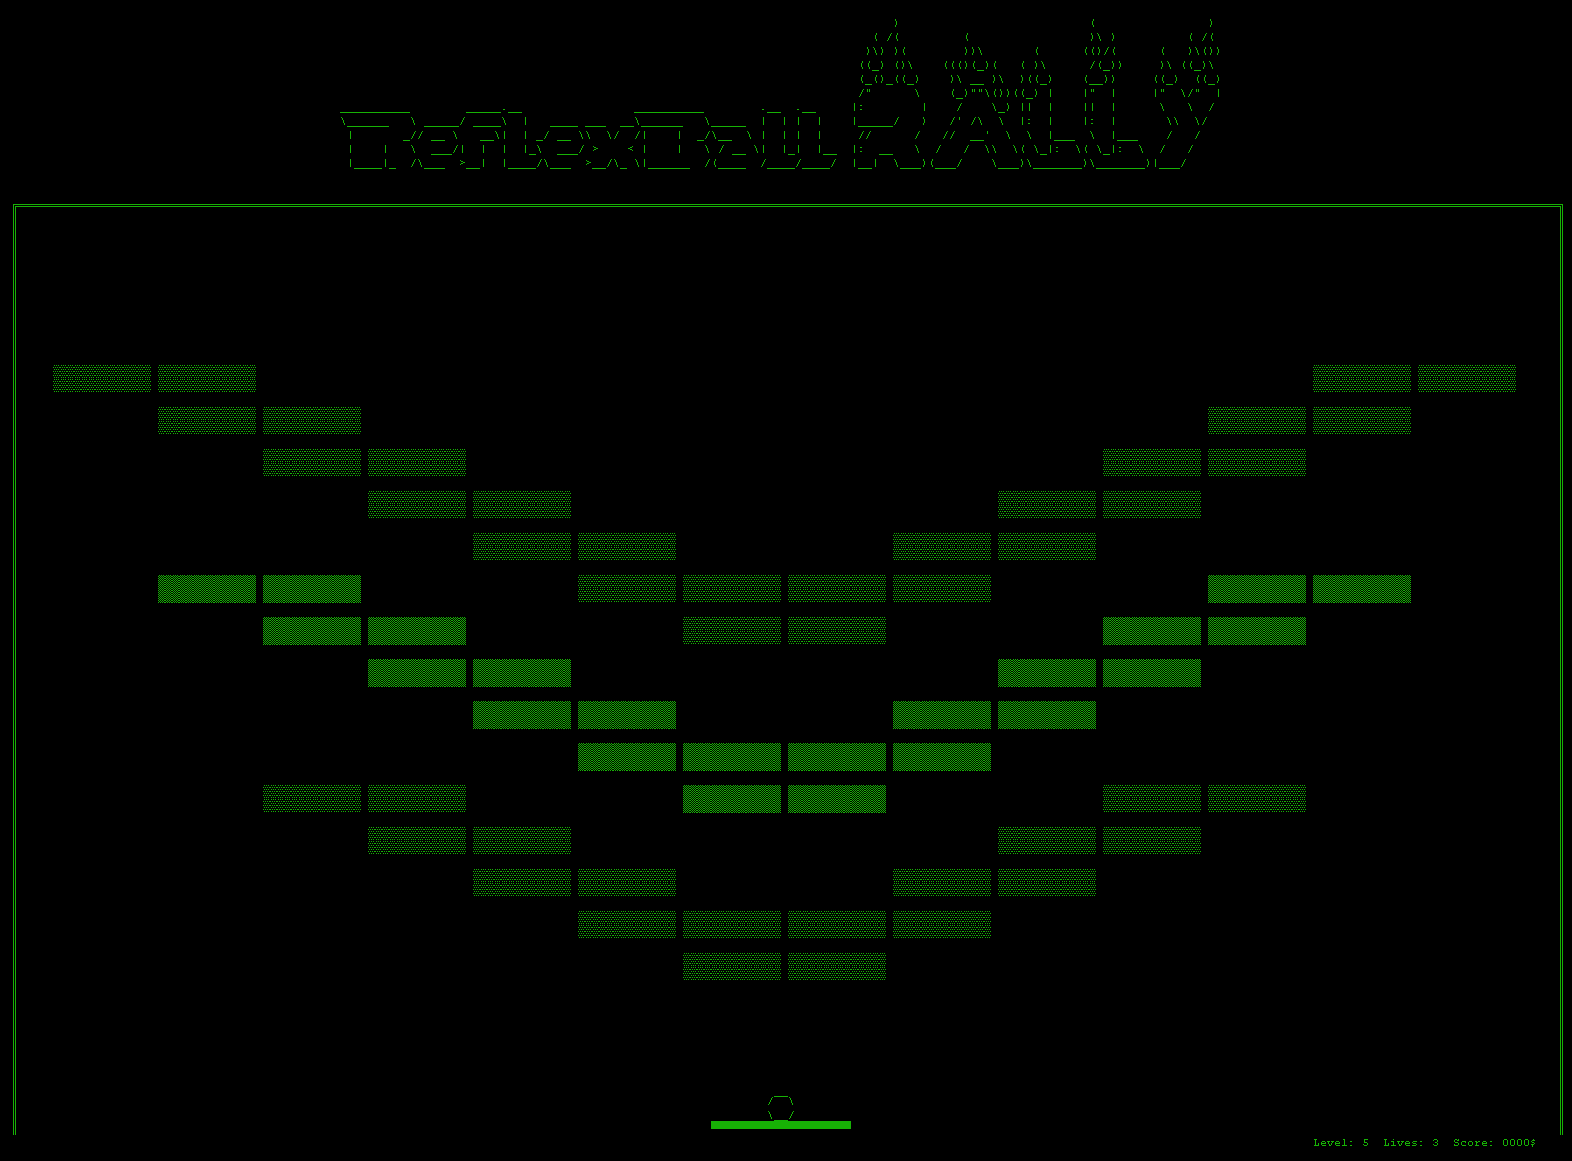
\includegraphics[width=\linewidth]{figs/screenshots/level5.png}
\caption{Level 5}
\label{fig:level5}
\end{minipage}\hfill
\begin{minipage}[b]{0.32\textwidth}
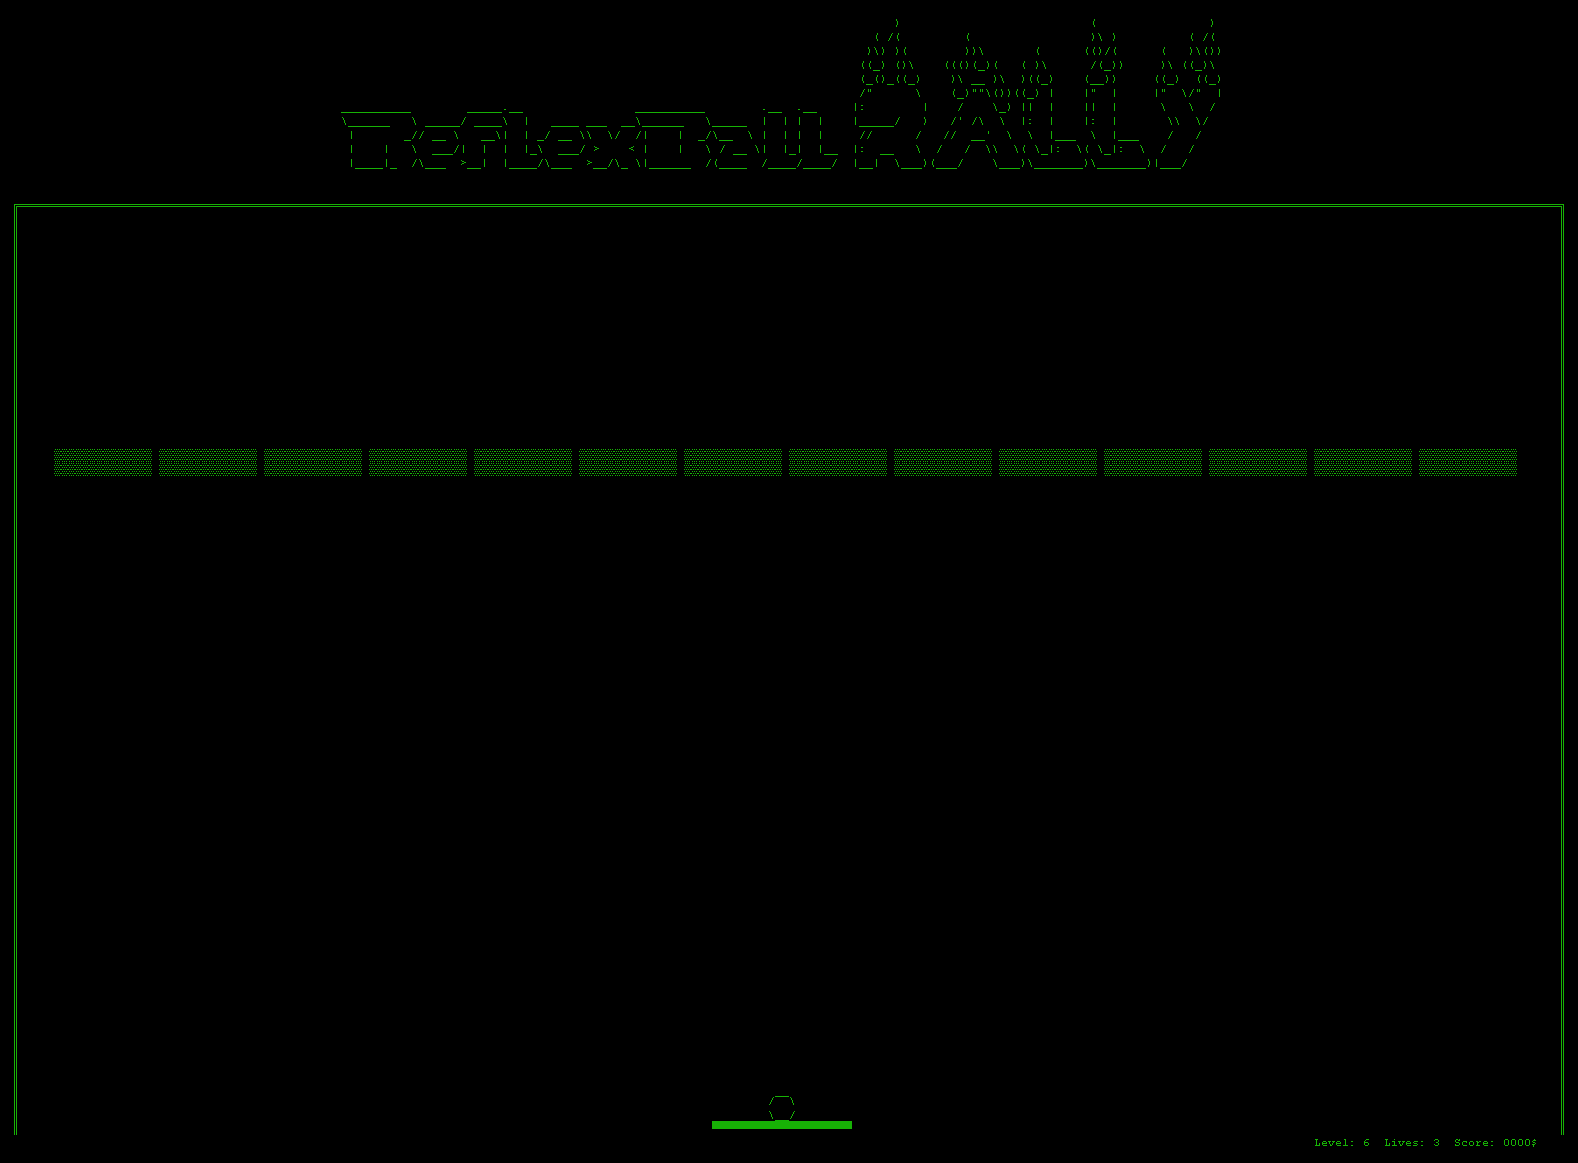
\includegraphics[width=\linewidth]{figs/screenshots/level6.png}
\caption{Level 6}
\label{fig:level6}
\end{minipage}\hfill
\end{figure}
\newpage
Hvis man taber spillet vises "Game Over!" skrevet med ASCII art, samt 1 tilfældig ud af 8 forskellige undertitler (som ikke nødvendigvis altid er hverken lige politisk korrekte eller venlige). Figur \ref{fig:gameover_2} viser et screenshot af dette. Bliver man Game Over vil LED displayet blive ved med at scrolle "Game Over" efterfulgt af ens score, indtil man klikker på en vilkårlig tast. Når dette gøres, kommer man tilbage til startmenuen.\\

\begin{figure}[h!]
\centering

\includegraphics[scale=0.25]{figs/screenshots/gameover_crop.png}
\caption{Eksempel på screenshot game over tekst}
\label{fig:gameover_2}
\end{figure}

Hvis man vinder spillet på Easy, Medium eller Hard vises et screenshot magen til figur \ref{fig:won_normal_2} som belønning for det hårde slid. Hvis man derimod skulle vinde spillet på sværhedsgraden Chuck Norris (hvis dette overhovedet kan lade sig gøre), fås en sølle belønning, da et ASCII-Art billede af Chuck Norris med underteksten "Only Chuck Norris wins Chuck Norris mode!" vises kort (se figur \ref{fig:won_chuck}), efterfulgt af at spillet vil starte forfra i level 1 på Chuck Norris mode.\\

\begin{figure}[h!]
\begin{minipage}[b]{0.49\textwidth}

\includegraphics[width=\linewidth]{figs/screenshots/won_normal.png}
\caption{Screenshot ved gennemførsel af spillet}
\label{fig:won_normal_2}
\end{minipage}\hfill
\begin{minipage}[b]{0.49\textwidth}

\includegraphics[width=\linewidth]{figs/screenshots/won_chuck_crop.png}
\caption{Screenshot ved gennemførsel af spillet i Chuck Norris mode}
\label{fig:won_chuck}
\end{minipage}\hfill
\end{figure}